\documentclass[twocolumn]{article}
\usepackage[utf8]{inputenc}

\usepackage{enumitem}
\usepackage{framed}
\usepackage{tabularx}
\usepackage{amsmath}
\usepackage{qtree}
\usepackage{geometry}
\usepackage{gb4e}
\usepackage{dblfloatfix}
\usepackage{graphicx}
\geometry{margin=1in}
\setlength{\belowcaptionskip}{-11pt}

\title{Why Do We Study Syntax?}
\begin{document}

You, and every adult human you know, are amazingly good at speaking. You could probably form sentences in your
sleep --- indeed, some of us do! Perhaps you can even speak in two different languages. However,
most people, when asked to explain how they form sentences, and how they judge whether a sentence sounds
right, have a very difficult time explaining their logic. We have a massive amount of subconscious
knowledge about language, and although we know how to speak, very rarely can we explain all that
knowledge to someone else in a precise form. Linguistics is the study of this subconscious
knowledge.

Syntax, a subfield of linguistics, is the study of the \emph{structure} of language, the study of
how words can be combined together into sentences. Some aspects of syntax may seem slightly familiar
from early schooling; for instance, you might explain that the sentence ``I dog'' is ungrammatical,
as it has no verb. However, real-world uses of language are much more complex. For instance, we know
that in colloquial English speech, the words ``want to'' are quite often replaced by ``wanna'';
however, while you can say ``Who do you want to kiss the puppy?'' (meaning ``Which person do you
think should kiss the puppy?''), the sentence ``Who do you wanna kiss the puppy?'' sounds
nonsensical to most native English speakers. While most schooling focuses on correctness of written
English, the phenomenon above happens in regular speech --- which is what the study of syntax seeks
to understand. 

In addition to explaining colloquialisms, syntacticians may study more common turns of phrase. For
example, syntactic theories can explain why ``I am quickly running'' (with adverb after verb) sounds
better (or at least more normal) than ``I quickly am running'' (with adverb before verb), even
though ``I quickly sing'' and ``I sing quickly'' both sound perfectly fine. They can also explain
why the phrase ``the student of physics with the pink mohawk'' sounds reasonable (if strange), while
``the student with the pink mohawk of physics'' sounds absolutely absurd (even though all we've done
is changed the order of some prepositional phrases relating to ``the student''). In summary, syntax
is not just the study of grammar --- instead, it's the study of how \emph{real} language is
structured, and aims to understand the rules that govern which sentences are valid and how these
sentences are constructed.

This distinction is known as ``descriptive'' (as opposed to ``prescriptive'') grammar; one could
describe syntax as studying descriptive grammar. The term \textbf{grammar} usually refers to
prescriptive grammar, which is a set of rules that people are \emph{supposed} to follow in speech
and writing; descriptive grammar, however, is the set of rules that people \emph{really} follow. For
instance, while in prescriptive grammar, a noun might be described as ``a person, place, thing, or
idea'', the descriptive grammar approach simply states that a noun is any word which can take the
place of noun-like thing --- for instance, any word that follows the determiner ``the''. (A concrete
difference can be demonstrated via the word ``of'': everything that follows ``of'' can behave like
a noun, so a descriptivist would say that ``running'' in ``practice of running'' is a noun, while a
prescriptivist might say that it is a verb, since ``run'' is a verb.) Like prescriptive grammar,
however, descriptive grammar claims that language is governed by fixed rules which speakers follow.

Since syntacticians are concerned with real-world language, their investigative methods rely on
native speaker judgements of grammaticality. For instance, syntacticians have a concept of a
``constituent''; several worlds that form one logical unit in the speakers minds. For example, ``the
student of physics'' and ``running quickly'' are both constituents, while ``the student of'' and
``from the'' are not. In order to determine whether a phrase is a constituent, syntacticians will
ask native speakers for judgements about the grammaticality of special constructed sentences known
as \emph{constituent tests}. Although there are a number of constituent tests, they all rely on the
same basic idea: that you can construct a sentence around the potential constituent and if native
speakers think the constructed sentences sound find, the potential constituent is a true
constituent. For instance, in order to check for constituency of the phrase ``students of physics'',
native speakers will be asked about the grammaticality of sentences such as ``It was students of
physics that we saw'', ``Students of physics is what we saw'', and ``We saw them'' (with ``them''
meaning ``students of physics''). In this case, the constituent tests would determine that
``students of physics'' are a constituent. However, suppose a syntactician wanted to know whether
``running with'' in the sentence ``He was running with his friend'' was a constituent. Then, they
might ask about the grammaticality of sentences such as ``It was running with that he did his
friend'' or ``He did that his friend'' (with ``did that'' taking the place of ``running with'');
since all of these sound wrong to native speakers, the syntactician would conclude that ``running
with'' is not a single logical unit in the speakers minds, and thus is not a constituent. The key
point to note here is not the constituent tests themselves, but rather that syntacticians regularly
use native speaker judgements and intuitions as their data, and try to explain these intuitions
rigorously.

Though the data are based on speaker intuitions, the analyses of these data are quite rigorous.
Although many approaches exist to syntactic analysis, many syntacticians hold with something known
as \textbf{generative grammar}. The fundamental tenet of generative grammar is that there exists a
set of rules which can predict, or generate, all valid sentences in the speaker's language. These
rules can come in many forms, but a prevalent representation is one of \textbf{phrase structure
rules} and \textbf{transformation rules}. 

We won't get in to the details of either, but we will note
the main ideas. Phrase structure rules govern the ordering of words by positing that language
possesses a very regular underlying tree structure. A tree structure indicates heirarchical
relationships, just like a family tree; the very last things on the tree (like the last generation
on a family tree) are the words themselves, and the intermediate levels (like parents on a family
tree) are different concepts.  For instance, verb phrases when represented in this tree form will
have two children: a subject and the verb itself. In some cases, the verb itself will have its own
children, consisting of the main verb word and things such as its direct and indirect objects or
prepositions describing its actions. Syntacticians can then represent these trees graphically to
analyze them, as demonstrated in figure~\ref{extree}.

\begin{center}
    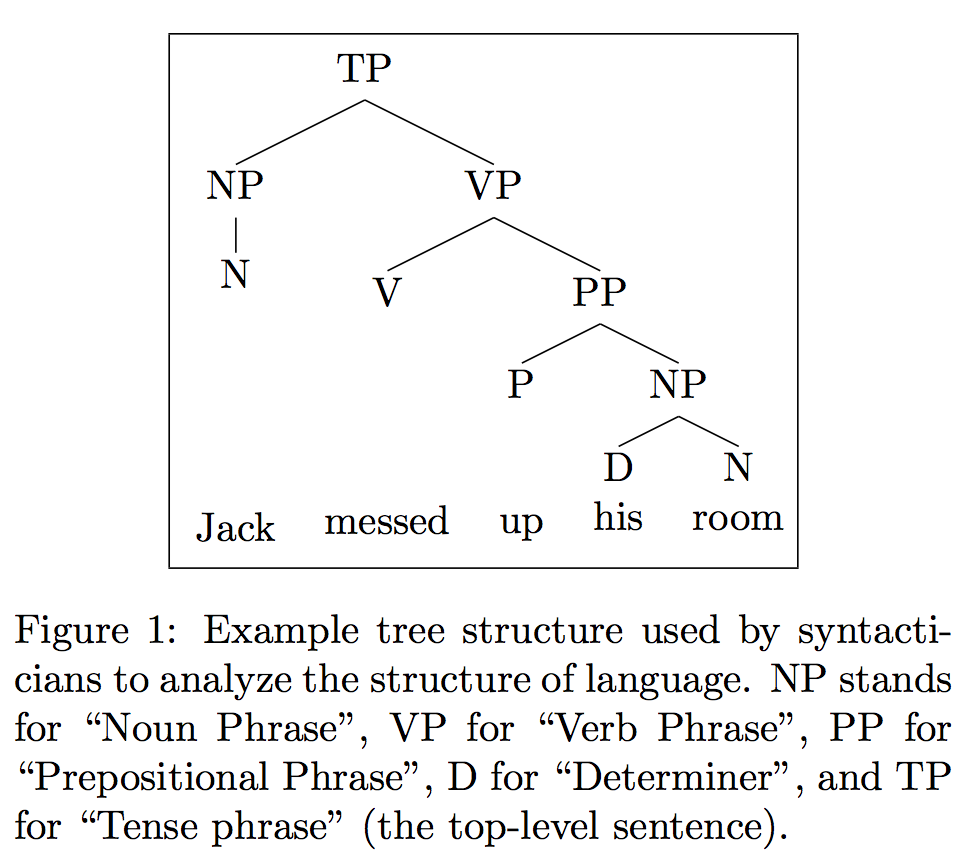
\includegraphics[scale=0.5]{images/sample-tree.png}
\end{center}

However, these trees are sometimes insufficient to explain all language. In order to rectify this,
syntacticians use transformation rules. Transformation rules are rules which dictate that while the
deep underlying structure of language is trees such as the ones generated by phrase, the things that
people actually say are a bit different. This difference is encoded by rules which operate on these
underlying trees by moving parts of them around. For instance, these rules can move certain noun
phrases higher up in the tree, or cause verbs to move earlier in the sentence. 

As an aside, that's why ``I quickly ran'' sounds fine but ``I quickly am running'' sounds a bit
strange; there's a rule which dictates that some verbs, including ``to be'', must move to be right
after the subject of the sentence. If this rule is obeyed, the ``am'' in ``quickly am running''
would move to be after the ``I'', yielding ``I am quickly running''. Thus, the fact that ``I quickly
am running'' sounds strange because it is a violation of this transformation rule!

It turns out that just like these phrase structure rules and transformation rules can explain the
puzzle of ``I quickly am running'', they do a fairly good job of explaining the other puzzles
introduced earlier, as well as many others. In addition, these rules are very surprisingly regular
across languages --- even languages which seem thoroughly different, such as English, Irish, Hebrew,
and Japanese, have many almost identical phrase structure and transformation rules. This incredible
observation points to an underlying connection --- since even languages which are historically
unrelated share many of these rules, linguists have posited the existence of a \textbf{universal
grammar}, a grammar somehow inherent to the human brain. This theory has been debated for a long
time; if this is true, however, then the study of syntax pertains to very deep psychological
phenomena.  Our languages are an integral portion of ourselves and our intelligence, so in the
process of studying and understanding their structure we inevitably gain a greater understanding of
ourselves.

\end{document}
